% updated April 2002 by Antje Endemann
% Based on CVPR 07 and LNCS, with modifications by DAF, AZ and elle, 2008 and AA, 2010, and CC, 2011; TT, 2014; AAS, 2016; AAS, 2020

\documentclass[runningheads]{llncs}
\usepackage{graphicx}
\usepackage{comment}
\usepackage{amsmath,amssymb} % define this before the line numbering.
\usepackage{color}

% INITIAL SUBMISSION - The following two lines are NOT commented
% CAMERA READY - Comment OUT the following two lines
\usepackage{ruler}
\usepackage[width=122mm,left=12mm,paperwidth=146mm,height=193mm,top=12mm,paperheight=217mm]{geometry}

\usepackage{amsmath}
\usepackage{amssymb}
\usepackage{mathrsfs}
\usepackage{amssymb}
\usepackage{multirow}
\usepackage{subfigure}
\usepackage{booktabs}
\usepackage{floatrow}
\graphicspath{{pic/}}

% Include other packages here, before hyperref.

% If you comment hyperref and then uncomment it, you should delete
% egpaper.aux before re-running latex.  (Or just hit 'q' on the first latex
% run, let it finish, and you should be clear).
\usepackage[pagebackref=true,breaklinks=true,letterpaper=true,colorlinks,bookmarks=false]{hyperref}


\begin{document}
% \renewcommand\thelinenumber{\color[rgb]{0.2,0.5,0.8}\normalfont\sffamily\scriptsize\arabic{linenumber}\color[rgb]{0,0,0}}
% \renewcommand\makeLineNumber {\hss\thelinenumber\ \hspace{6mm} \rlap{\hskip\textwidth\ \hspace{6.5mm}\thelinenumber}}
% \linenumbers
\pagestyle{headings}
\mainmatter
\def\ECCVSubNumber{100}  % Insert your submission number here

\title{Author Guidelines for ECCV Submission} % Replace with your title

% INITIAL SUBMISSION 
%\begin{comment}
\titlerunning{ECCV-20 submission ID \ECCVSubNumber} 
\authorrunning{ECCV-20 submission ID \ECCVSubNumber} 
\author{Anonymous ECCV submission}
\institute{Paper ID \ECCVSubNumber}
%\end{comment}
%******************

% CAMERA READY SUBMISSION
\begin{comment}
\titlerunning{Abbreviated paper title}
% If the paper title is too long for the running head, you can set
% an abbreviated paper title here
%
\author{First Author\inst{1}\orcidID{0000-1111-2222-3333} \and
Second Author\inst{2,3}\orcidID{1111-2222-3333-4444} \and
Third Author\inst{3}\orcidID{2222--3333-4444-5555}}
%
\authorrunning{F. Author et al.}
% First names are abbreviated in the running head.
% If there are more than two authors, 'et al.' is used.
%
\institute{Princeton University, Princeton NJ 08544, USA \and
Springer Heidelberg, Tiergartenstr. 17, 69121 Heidelberg, Germany
\email{lncs@springer.com}\\
\url{http://www.springer.com/gp/computer-science/lncs} \and
ABC Institute, Rupert-Karls-University Heidelberg, Heidelberg, Germany\\
\email{\{abc,lncs\}@uni-heidelberg.de}}
\end{comment}
%******************
\maketitle

\begin{abstract}
The abstract should summarize the contents of the paper. LNCS guidelines
indicate it should be at least 70 and at most 150 words. It should be set in 9-point
font size and should be inset 1.0~cm from the right and left margins.
\dots
\keywords{We would like to encourage you to list your keywords within
the abstract section}
\end{abstract}


\section{Introduction}


This document serves as an example submission. It illustrates the format
we expect authors to follow when submitting a paper to ECCV. 
At the same time, it gives details on various aspects of paper submission,
including preservation of anonymity and how to deal with dual submissions,
so we advise authors to read this document carefully.

\section{Initial Submission}

\subsection{Language}

All manuscripts must be in English.

\subsection{Paper length}
Papers submitted for review should be complete. 
The length should match that intended for final publication. 
Papers accepted for the conference will be allocated 14 pages (plus references) in the proceedings. 
Note that the allocated 14 pages do not include the references. The reason for this policy
is that we do not want authors to omit references for sake of space limitations.

Papers with more than 14 pages (excluding references) will be rejected without review.
This includes papers where the margins and
formatting are deemed to have been significantly altered from those
laid down by this style guide.  The reason such papers will not be reviewed is that there is no provision for supervised revisions of manuscripts. The reviewing process cannot determine the suitability of the paper for presentation in 14 pages if it is reviewed in 16.

\subsection{Paper ID}

It is imperative that the paper ID is mentioned on each page of the manuscript.
The paper ID is a number automatically assigned to your submission when 
registering your paper submission on the submission site.

%\subsection{Line numbering}

All lines should be numbered in the initial submission, as in this example document. This makes reviewing more efficient, because reviewers can refer to a line on a page. Line numbering is removed in the camera-ready.


\subsection{Mathematics}

Please number all of your sections and displayed equations.  Again,
this makes reviewing more efficient, because reviewers can refer to a
line on a page.  Also, it is important for readers to be able to refer
to any particular equation.  Just because you didn't refer to it in
the text doesn't mean some future reader might not need to refer to
it.  It is cumbersome to have to use circumlocutions like ``the
equation second from the top of page 3 column 1''.  (Note that the
line numbering will not be present in the final copy, so is not an
alternative to equation numbers).  Some authors might benefit from
reading Mermin's description of how to write mathematics:
\url{www.pamitc.org/documents/mermin.pdf}.
\section{Policies}
\subsection{Review Process}
By submitting a paper to ECCV, the authors agree to the review process and understand that papers are processed by the Toronto system to match each manuscript to the best possible chairs and reviewers.
\subsection{Confidentiality}
The review process of ECCV is confidential. Reviewers are volunteers not part of the ECCV organisation and their efforts are greatly appreciated. The standard practice of keeping all information confidential during the review is part of the standard communication to all reviewers. Misuse of confidential information is a severe professional failure and  appropriate measures will be taken when brought to the attention of ECCV organizers. It should be noted, however, that the organisation of ECCV is not and cannot be held responsible for the consequences when reviewers break confidentiality.

Accepted papers will be published by Springer (with appropriate copyrights) electronically up to three weeks prior to the main conference. Please make sure to discuss this issue with your legal advisors as it pertains to public disclosure of the contents of the papers submitted.
\subsection{Dual and Double Submissions}
By submitting a manuscript to ECCV 2020, authors acknowledge that it has not been previously published or accepted for publication in substantially similar form in any peer-reviewed venue including journal, conference, or workshop. Furthermore, no paper substantially similar in content has been or will be submitted to a journal, another conference or workshop during the review period (March 05, 2020 – July 3, 2020). The authors also attest that they did not submit substantially similar submissions to ECCV 2020. Violation of any of these conditions will lead to rejection and the violation will be reported to the other venue or journal, which will typically lead to rejection there as well. 

The goals of the dual submission policy are (i) to have exciting new work be published for the first time at ECCV 2020, and (ii) to avoid duplicating the efforts of the reviewers.
Therefore, all papers under review are checked for dual submissions and this is not allowed, independent of the page size of submissions. 

For already published papers, our policy is based upon the following particular definition of ``publication''. A publication, for the purposes of the dual submission policy, is defined to be a written work longer than four pages that was submitted for review by peers for either acceptance or rejection, and, after review, was accepted. In particular, this definition of publication does not depend upon whether such an accepted written work appears in a formal proceedings or whether the organizers declare that such work ``counts as a publication''. 

An arXiv.org paper does not count as a publication because it was not peer-reviewed for acceptance. The same is true for university technical reports. However, this definition of publication does include peer-reviewed workshop papers, even if they do not appear in a proceedings, if their length is more than 4 pages including citations. Given this definition, any submission to ECCV 2020 should not have substantial overlap with prior publications or other concurrent submissions. As a rule of thumb, the ECCV 2020 submission should contain no more than 20 percent of material from previous publications. 

\subsection{Requirements for publication}
Publication of the paper in the ECCV 2020 proceedings of Springer requires that at least one of the authors registers for the conference and present the paper there. It also requires that a camera-ready version that satisfies all formatting requirements is submitted before the camera-ready deadline. 
\subsection{Double blind review}
\label{sec:blind}
ECCV reviewing is double blind, in that authors do not know the names of the area chair/reviewers of their papers, and the area chairs/reviewers cannot, beyond reasonable doubt, infer the names of the authors from the submission and the additional material. Avoid providing links to websites that identify the authors. Violation of any of these guidelines may lead to rejection without review. If you need to cite a different paper of yours that is being submitted concurrently to ECCV, the authors should (1) cite these papers, (2) argue in the body of your paper why your ECCV paper is non trivially different from these concurrent submissions, and (3) include anonymized versions of those papers in the supplemental material.

Many authors misunderstand the concept of anonymizing for blind
review. Blind review does not mean that one must remove
citations to one's own work. In fact it is often impossible to
review a paper unless the previous citations are known and
available.

Blind review means that you do not use the words ``my'' or ``our''
when citing previous work.  That is all.  (But see below for
technical reports).

Saying ``this builds on the work of Lucy Smith [1]'' does not say
that you are Lucy Smith, it says that you are building on her
work.  If you are Smith and Jones, do not say ``as we show in
[7]'', say ``as Smith and Jones show in [7]'' and at the end of the
paper, include reference 7 as you would any other cited work.

An example of a bad paper:
\begin{quote}
\begin{center}
    An analysis of the frobnicatable foo filter.
\end{center}

   In this paper we present a performance analysis of our
   previous paper [1], and show it to be inferior to all
   previously known methods.  Why the previous paper was
   accepted without this analysis is beyond me.

   [1] Removed for blind review
\end{quote}


An example of an excellent paper:

\begin{quote}
\begin{center}
     An analysis of the frobnicatable foo filter.
\end{center}

   In this paper we present a performance analysis of the
   paper of Smith [1], and show it to be inferior to
   all previously known methods.  Why the previous paper
   was accepted without this analysis is beyond me.

   [1] Smith, L. and Jones, C. ``The frobnicatable foo
   filter, a fundamental contribution to human knowledge''.
   Nature 381(12), 1-213.
\end{quote}

If you are making a submission to another conference at the same
time, which covers similar or overlapping material, you may need
to refer to that submission in order to explain the differences,
just as you would if you had previously published related work. In
such cases, include the anonymized parallel
submission~\cite{Authors14} as additional material and cite it as
\begin{quote}
1. Authors. ``The frobnicatable foo filter'', BMVC 2014 Submission
ID 324, Supplied as additional material {\tt bmvc14.pdf}.
\end{quote}

Finally, you may feel you need to tell the reader that more
details can be found elsewhere, and refer them to a technical
report.  For conference submissions, the paper must stand on its
own, and not {\em require} the reviewer to go to a techreport for
further details.  Thus, you may say in the body of the paper
``further details may be found in~\cite{Authors14b}''.  Then
submit the techreport as additional material. Again, you may not
assume the reviewers will read this material.

Sometimes your paper is about a problem which you tested using a tool which
is widely known to be restricted to a single institution.  For example,
let's say it's 1969, you have solved a key problem on the Apollo lander,
and you believe that the ECCV audience would like to hear about your
solution.  The work is a development of your celebrated 1968 paper entitled
``Zero-g frobnication: How being the only people in the world with access to
the Apollo lander source code makes us a wow at parties'', by Zeus.

You can handle this paper like any other.  Don't write ``We show how to
improve our previous work [Anonymous, 1968].  This time we tested the
algorithm on a lunar lander [name of lander removed for blind review]''.
That would be silly, and would immediately identify the authors. Instead
write the following:
\begin{quotation}
\noindent
   We describe a system for zero-g frobnication.  This
   system is new because it handles the following cases:
   A, B.  Previous systems [Zeus et al. 1968] didn't
   handle case B properly.  Ours handles it by including
   a foo term in the bar integral.

   ...

   The proposed system was integrated with the Apollo
   lunar lander, and went all the way to the moon, don't
   you know.  It displayed the following behaviours
   which show how well we solved cases A and B: ...
\end{quotation}
As you can see, the above text follows standard scientific convention,
reads better than the first version, and does not explicitly name you as
the authors.  A reviewer might think it likely that the new paper was
written by Zeus, but cannot make any decision based on that guess.
He or she would have to be sure that no other authors could have been
contracted to solve problem B. \\

For sake of anonymity, it's recommended to omit acknowledgements
in your review copy. They can be added later when you prepare the final copy.

\section{Manuscript Preparation}

This is an edited version of Springer LNCS instructions adapted
for ECCV 2020 first paper submission.
You are strongly encouraged to use \LaTeX2$_\varepsilon$ for the
preparation of your
camera-ready manuscript together with the corresponding Springer
class file \verb+llncs.cls+.

We would like to stress that the class/style files and the template
should not be manipulated and that the guidelines regarding font sizes
and format should be adhered to. This is to ensure that the end product
is as homogeneous as possible.

\subsection{Printing Area}
The printing area is $122  \; \mbox{mm} \times 193 \;
\mbox{mm}$.
The text should be justified to occupy the full line width,
so that the right margin is not ragged, with words hyphenated as
appropriate. Please fill pages so that the length of the text
is no less than 180~mm.

\subsection{Layout, Typeface, Font Sizes, and Numbering}
Use 10-point type for the name(s) of the author(s) and 9-point type for
the address(es) and the abstract. For the main text, please use 10-point
type and single-line spacing.
We recommend using Computer Modern Roman (CM) fonts, Times, or one
of the similar typefaces widely used in photo-typesetting.
(In these typefaces the letters have serifs, i.e., short endstrokes at
the head and the foot of letters.)
Italic type may be used to emphasize words in running text. Bold
type and underlining should be avoided.
With these sizes, the interline distance should be set so that some 45
lines occur on a full-text page.

\subsubsection{Headings.}

Headings should be capitalized
(i.e., nouns, verbs, and all other words
except articles, prepositions, and conjunctions should be set with an
initial capital) and should,
with the exception of the title, be aligned to the left.
Words joined by a hyphen are subject to a special rule. If the first
word can stand alone, the second word should be capitalized.
The font sizes
are given in Table~\ref{table:headings}.
\setlength{\tabcolsep}{4pt}
\begin{table}
\begin{center}
\caption{Font sizes of headings. Table captions should always be
positioned {\it above} the tables. The final sentence of a table
caption should end without a full stop}
\label{table:headings}
\begin{tabular}{lll}
\hline\noalign{\smallskip}
Heading level & Example & Font size and style\\
\noalign{\smallskip}
\hline
\noalign{\smallskip}
Title (centered)  & {\Large \bf Lecture Notes \dots} & 14 point, bold\\
1st-level heading & {\large \bf 1 Introduction} & 12 point, bold\\
2nd-level heading & {\bf 2.1 Printing Area} & 10 point, bold\\
3rd-level heading & {\bf Headings.} Text follows \dots & 10 point, bold
\\
4th-level heading & {\it Remark.} Text follows \dots & 10 point,
italic\\
\hline
\end{tabular}
\end{center}
\end{table}
\setlength{\tabcolsep}{1.4pt}

Here are some examples of headings: ``Criteria to Disprove Context-Freeness of
Collage Languages'', ``On Correcting the Intrusion of Tracing
Non-deterministic Programs by Software'', ``A User-Friendly and
Extendable Data Distribution System'', ``Multi-flip Networks:
Parallelizing GenSAT'', ``Self-determinations of Man''.

\subsubsection{Lemmas, Propositions, and Theorems.}

The numbers accorded to lemmas, propositions, and theorems etc. should
appear in consecutive order, starting with the number 1, and not, for
example, with the number 11.

\subsection{Figures and Photographs}
\label{sect:figures}

Please produce your figures electronically and integrate
them into your text file. For \LaTeX\ users we recommend using package
\verb+graphicx+ or the style files \verb+psfig+ or \verb+epsf+.

Check that in line drawings, lines are not
interrupted and have constant width. Grids and details within the
figures must be clearly readable and may not be written one on top of
the other. Line drawings should have a resolution of at least 800 dpi
(preferably 1200 dpi).
For digital halftones 300 dpi is usually sufficient.
The lettering in figures should have a height of 2~mm (10-point type).
Figures should be scaled up or down accordingly.
Please do not use any absolute coordinates in figures.

Figures should be numbered and should have a caption which should
always be positioned {\it under} the figures, in contrast to the caption
belonging to a table, which should always appear {\it above} the table.
Please center the captions between the margins and set them in
9-point type
(Fig.~\ref{fig:example} shows an example).
The distance between text and figure should be about 8~mm, the
distance between figure and caption about 5~mm.
\begin{figure}
\centering
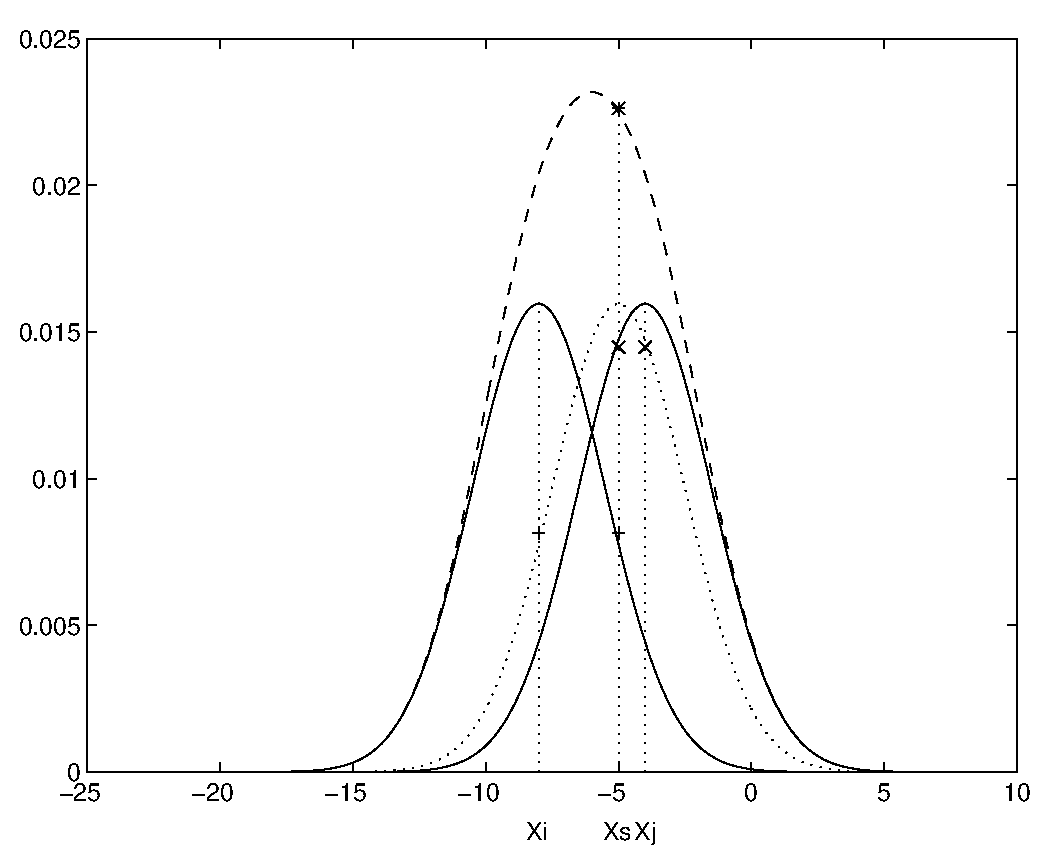
\includegraphics[height=6.5cm]{eijkel2}
\caption{One kernel at $x_s$ ({\it dotted kernel}) or two kernels at
$x_i$ and $x_j$ ({\it left and right}) lead to the same summed estimate
at $x_s$. This shows a figure consisting of different types of
lines. Elements of the figure described in the caption should be set in
italics,
in parentheses, as shown in this sample caption. The last
sentence of a figure caption should generally end without a full stop}
\label{fig:example}
\end{figure}

If possible (e.g. if you use \LaTeX) please define figures as floating
objects. \LaTeX\ users, please avoid using the location
parameter ``h'' for ``here''. If you have to insert a pagebreak before a
figure, please ensure that the previous page is completely filled.


\subsection{Formulas}

Displayed equations or formulas are centered and set on a separate
line (with an extra line or halfline space above and below). Displayed
expressions should be numbered for reference. The numbers should be
consecutive within the contribution,
with numbers enclosed in parentheses and set on the right margin.
For example,
\begin{align}
  \psi (u) & = \int_{0}^{T} \left[\frac{1}{2}
  \left(\Lambda_{0}^{-1} u,u\right) + N^{\ast} (-u)\right] dt \; \\
& = 0 ?
\end{align}

Please punctuate a displayed equation in the same way as ordinary
text but with a small space before the end punctuation.

\subsection{Footnotes}

The superscript numeral used to refer to a footnote appears in the text
either directly after the word to be discussed or, in relation to a
phrase or a sentence, following the punctuation sign (comma,
semicolon, or full stop). Footnotes should appear at the bottom of
the
normal text area, with a line of about 2~cm in \TeX\ and about 5~cm in
Word set
immediately above them.\footnote{The footnote numeral is set flush left
and the text follows with the usual word spacing. Second and subsequent
lines are indented. Footnotes should end with a full stop.}


\subsection{Program Code}

Program listings or program commands in the text are normally set in
typewriter font, e.g., CMTT10 or Courier.

\noindent
{\it Example of a Computer Program}
\begin{verbatim}
program Inflation (Output)
  {Assuming annual inflation rates of 7%, 8%, and 10%,...
   years};
   const
     MaxYears = 10;
   var
     Year: 0..MaxYears;
     Factor1, Factor2, Factor3: Real;
   begin
     Year := 0;
     Factor1 := 1.0; Factor2 := 1.0; Factor3 := 1.0;
     WriteLn('Year  7% 8% 10%'); WriteLn;
     repeat
       Year := Year + 1;
       Factor1 := Factor1 * 1.07;
       Factor2 := Factor2 * 1.08;
       Factor3 := Factor3 * 1.10;
       WriteLn(Year:5,Factor1:7:3,Factor2:7:3,Factor3:7:3)
     until Year = MaxYears
end.
\end{verbatim}
%
\noindent
{\small (Example from Jensen K., Wirth N. (1991) Pascal user manual and
report. Springer, New York)}



\subsection{Citations}

The list of references is headed ``References" and is not assigned a
number
in the decimal system of headings. The list should be set in small print
and placed at the end of your contribution, in front of the appendix,
if one exists.
Please do not insert a pagebreak before the list of references if the
page is not completely filled.
An example is given at the
end of this information sheet. For citations in the text please use
square brackets and consecutive numbers: \cite{Alpher02},
\cite{Alpher03}, \cite{Alpher04} \dots

\section{Submitting a Camera-Ready for an Accepted Paper}
\subsection{Converting Initial Submission to Camera-Ready}
To convert a submission file into a camera-ready for an accepted paper:
\begin{enumerate}
    \item  First comment out \begin{verbatim}
        \usepackage{ruler}
    \end{verbatim} and the line that follows it.
    \item  The anonymous title part should be removed or commented out, and a proper author block should be inserted, for which a skeleton is provided in a commented-out version. These are marked in the source file as \begin{verbatim}
        % INITIAL SUBMISSION 
    \end{verbatim} and \begin{verbatim}
        % CAMERA READY SUBMISSION 
    \end{verbatim}
    \item Please write out author names in full in the paper, i.e. full given and family names. If any authors have names that can be parsed into FirstName LastName in multiple ways, please include the correct parsing in a comment to the editors, below the \begin{verbatim}\author{}\end{verbatim} field.
    \item Make sure you have inserted the proper Acknowledgments.
  \end{enumerate}  
 
\subsection{Preparing the Submission Package}
We need all the source files (LaTeX files, style files, special fonts, figures, bib-files) that are required to compile papers, as well as the camera ready PDF. For each paper, one ZIP-file called XXXX.ZIP (where XXXX is the zero-padded, four-digit paper ID) has to be prepared and submitted via the ECCV 2020 Submission Website, using the password you received with your initial registration on that site. The size of the ZIP-file may not exceed the limit of 60 MByte. The ZIP-file has to contain the following:
  \begin{enumerate}
 \item  All source files, e.g. LaTeX2e files for the text, PS/EPS or PDF/JPG files for all figures.
 \item PDF file named ``XXXX.pdf" that has been produced by the submitted source, where XXXX is the four-digit paper ID (zero-padded if necessary). For example, if your paper ID is 24, the filename must be 0024.pdf. This PDF will be used as a reference and has to exactly match the output of the compilation.
 \item PDF file named ``XXXX-copyright.PDF": a scanned version of the signed copyright form (see ECCV 2020 Website, Camera Ready Guidelines for the correct form to use). 
 \item If you wish to provide supplementary material, the file name must be in the form XXXX-supp.pdf or XXXX-supp.zip, where XXXX is the zero-padded, four-digit paper ID as used in the previous step. Upload your supplemental file on the ``File Upload" page as a single PDF or ZIP file of 100 MB in size or less. Only PDF and ZIP files are allowed for supplementary material. You can put anything in this file – movies, code, additional results, accompanying technical reports–anything that may make your paper more useful to readers.  If your supplementary material includes video or image data, you are advised to use common codecs and file formats.  This will make the material viewable by the largest number of readers (a desirable outcome). ECCV encourages authors to submit videos using an MP4 codec such as DivX contained in an AVI. Also, please submit a README text file with each video specifying the exact codec used and a URL where the codec can be downloaded. Authors should refer to the contents of the supplementary material appropriately in the paper.
 \end{enumerate}

Check that the upload of your file (or files) was successful either by matching the file length to that on your computer, or by using the download options that will appear after you have uploaded. Please ensure that you upload the correct camera-ready PDF–renamed to XXXX.pdf as described in the previous step as your camera-ready submission. Every year there is at least one author who accidentally submits the wrong PDF as their camera-ready submission.

Further considerations for preparing the camera-ready package:
  \begin{enumerate}
    \item Make sure to include any further style files and fonts you may have used.
    \item References are to be supplied as BBL files to avoid omission of data while conversion from BIB to BBL.
    \item Please do not send any older versions of papers. There should be one set of source files and one XXXX.pdf file per paper. Our typesetters require the author-created pdfs in order to check the proper representation of symbols, figures, etc.
    \item  Please remove unnecessary files (such as eijkel2.pdf and eijkel2.eps) from the source folder. 
    \item  You may use sub-directories.
    \item  Make sure to use relative paths for referencing files.
    \item  Make sure the source you submit compiles.
\end{enumerate}

Springer is the first publisher to implement the ORCID identifier for proceedings, ultimately providing authors with a digital identifier that distinguishes them from every other researcher. ORCID (Open Researcher and Contributor ID) hosts a registry of unique researcher identifiers and a transparent method of linking research activities to these identifiers. This is achieved through embedding ORCID identifiers in key workflows, such as research profile maintenance, manuscript submissions, grant applications and patent applications.
\subsection{Most Frequently Encountered Issues}
Please kindly use the checklist below to deal with some of the most frequently encountered issues in ECCV submissions.

{\bf FILES:}
\begin{itemize}
    \item My submission package contains ONE compiled pdf file for the camera-ready version to go on Springerlink.
\item I have ensured that the submission package has all the additional files necessary for compiling the pdf on a standard LaTeX distribution.
\item I have used the correct copyright form (with editor names pre-printed), and a signed pdf is included in the zip file with the correct file name.
\end{itemize}

{\bf CONTENT:}
\begin{itemize}
\item I have removed all \verb \vspace  and \verb \hspace  commands from my paper.
\item I have not used \verb \thanks  or \verb \footnote  commands and symbols for corresponding authors in the title (which is processed with scripts) and (optionally) used an Acknowledgement section for all the acknowledgments, at the end of the paper.
\item I have not used \verb \cite  command in the abstract.
\item I have read the Springer author guidelines, and complied with them, including the point on providing full information on editors and publishers for each reference in the paper (Author Guidelines – Section 2.8).
\item I have entered a correct \verb \titlerunning{}  command and selected a meaningful short name for the paper.
\item I have entered \verb \index{Lastname,Firstname}  commands for names that are longer than two words.
\item I have used the same name spelling in all my papers accepted to ECCV and ECCV Workshops.
\item I have inserted the ORCID identifiers of the authors in the paper header (see http://bit.ly/2H5xBpN for more information).
\item I have not decreased the font size of any part of the paper (except tables) to fit into 14 pages, I understand Springer editors will remove such commands.
\end{itemize}
{\bf SUBMISSION:}
\begin{itemize}
\item All author names, titles, and contact author information are correctly entered in the submission site.
\item The corresponding author e-mail is given.
\item At least one author has registered by the camera ready deadline.
\end{itemize}

\section{Experiments}
In this section, to verify our design of the module, we set a complete series of  ablation studies on two prevailing indoor datasets : SUN\_RGBD`\cite{SUN_RGBD} and SCanNet\cite{SCannet} . We also adopted the  metrics of mAP@0.25 for evaluation, which is the same with \cite{VoteNet,deepsliding} .     

%In this section, we first conduct series of ablation studies to verify our design philosophy of the backbone stage utilized in 3D object detection tasks. We provide detailed analysis on how large receptive fields help the overall performance. Next, various forms of feature aggregation are validated to show the efficiency of the proposed densely-connected structure. Then, full results on two standard benchmarks are reported to show that PointDiffusion outperforms other approaches and achieves new state-of-the-art.

\begin{figure*}
			\begin{minipage}{1\textwidth}
				\centering
				\includegraphics[width=1.0\linewidth]{Figures/vis-rf.pdf}
			\end{minipage}
    \caption{The visualization of enlarged receptive field and denser point sampling with increased stage of Dense Point ASPP and larger dilation rate}
    \label{fig:vis-rf}
\end{figure*}

\subsection{Dataset}
Contrary to the common belief, the 3D indoor scenes in reality are featured with dense scans of point clouds, objects with varing sizes and complex environment. Thus we choose to deploy our method on the representative indoor scenes: SUN RGB-D and SCanNet 

\textbf{SUN RGB-D} \cite{SUN_RGBD} for 3D indoor scene understanding consists of around 10k RGB-D images annotated with 64,595 oriented 3D bounding boxes for nearly 40 object categories. In this paper, following \cite{VoteNet} we split the train/test set and report 3D detection performance on the 10 most common categories. %. The SUN RGB-D V2 datasetis the latest version  with more accurate annotations.% Our experiments follow a standard evaluation protocol and are implemented on both two datasets.

\textbf{ScanNet} \cite{SCannet} provides a wider range of indoor scenes with more densely scanned objects compared with the SUN RGB-D dataset. We use the public training and testing split of 1205 and 312 scans respectively. Vertices from meshes are sampled as the input point clouds. Following the ground-truth annotation mentioned in \cite{VoteNet}, we predict axis-aligned 3D bounding boxes in this scenarios.

In experiment parts, we follow the same protocol as \cite{VoteNet} and use the metrics of mean average precision(mAP) at IoU threshold of 0.25 for evaluation.

\subsection{Implementation Details} 
\noindent\textbf{Overall Architecture}
We  plug our module with different setings on the VoteNet\cite{VoteNet}, the current SOTA algorithm for 3D detection on point clouds .So that the feature of the point set will be encoded by our module, then the voting module\cite{VoteNet} will select the keypoints of the objects and then group them into 3D boxes.

To make fair comparisons with the methods of the VoteNet\cite{VoteNet}, we keep almost every aspect of the details unchanged, including the configuration of the voting module, loss functions, vote aggregation  except the backbone. 

 

%We mainly follow the detection architecture proposed in VoteNet\cite{VoteNet}, also shown in Figure \ref{fig:DenseASPP}, which could be further divided into three key components, noted as feature learning backbone, voting and proposing module. For fair comparison, the configuration of voting and proposing module are kept unchanged. 

%For the backbone feature learning part, we design multiple variants to validate the best way to aggregate. Basically, during the early stage of backbone learning, one or more SA layers are first adopted to transform the input point cloud into subset of fixed point number since direct manipulation on the raw point cloud is usually computationally-heavy and time-consuming. To be strictly aligned with the point resolution of VoteNet, we manually design two critical stage, with prefixes noted as SA2 and SA3, to represent models utilize a chain of SA layers (SA1 and SA1-SA2 respectively) as transformers on point resolution. As we can see, the output number of points “SA3-“ based models are generally the same as the original VoteNet. Meanwhile for “SA2-“ based models, we could obtain doubled number of output points, thus gaining the potential to learn more meaningful point features from higher point resolution.
\begin{table}
\centering
        \scalebox{0.9}{
		\begin{tabular}{l|cccccc}
		   \toprule
		  	Seed Layer & SA2 & SA3& SA4 & FP1 & FP2 &FP3\\
		  	%\noalign{\smallskip}
			\midrule
			%\noalign{\smallskip}
			Point Resolution & 1024 & 512 & 256 & 512 & 1024 & 2048\\
			mAP & 51.2 & 56.3 & 55.1 & 56.6 & \textbf{57.7} &57.1\\
		  	
		  	\bottomrule
                	
			\end{tabular}
			}
			
	\caption{The performance of different levels of Feature map of Vote,quoted from Table 8 of \cite{VoteNet}. }
	\label{tab:votenet_experiment}
\end{table}


%Next, we implant the proposed PointDiffusion module to aggregate features from different fields of view of the input point sets. We should notice that regardless of their settings, PointDiffusion modules always output the same point resolution as the input, thus granting us great flexibility in stacking and combing different feature maps. In practices, We adopt three dilation rates of 3, 6, 12 to perform point convolution from different receptive fields. Accordingly, parameters of radius and the maximum grouping samples should be carefully considered as they will hugely impact the distribution of the neighbors to be aggregated. Consequently, we gradually increase the number of radius and neighboring points of retrieved, which is set as 0.8, 1.2, 1.6 and 16, 32, 64 respectively.

\noindent\textbf{Training and Inference}
To keep in abreast with the performance of \cite{VoteNet}, we adopt the same data augmentation methods and training strategies. Adam Optimizer [XXX] is utilized with an initial learning rate of 0.001. Learning rate is scheduled to be decayed by the factor of 0.1 after the 80 epoch and another 0.1 after 120 epochs. The whole model is trained on a single Titan X GPU.
During evaluation stage, we take the points of the entire scene as the input. With a single feed-forward path, the region proposals are generated by the neural nets and further post-processed by 3D NMS method.

\subsection{Ablation Studies}
In the experiment, we choose the features of SA2 and SA3 shown in Table \ref{tab:votenet_experiment} as the candidate of the basic feature for fair comparison with VoteNet \cite{VoteNet}. the SA4 layer is not suitable because it has only 256 points, meaning that there will be no voting process because the voting number of the module has exactly the same number.% As we can see clearly in Table \ref{tab:votenet_experiment} quoted from \cite{VoteNet}, the SA4 layer is not suitable for base feature because it has only 256 points, meaning that there will be no voting process because the voting number of the module has exactly the same number. The SA3 layer has a good performance of 56.1\% mAP on SUN RGB-D\_v1 thus making it a good candidate for base feature of the module, even though SA2 layer has only the performance of 51.2 mAP on the benchmark, it has the same point resolution with the feature of FP2, which has performed best in comparison with other levels of the features. Thus in the experiment, we choose the basic features of SA2 and SA3 layers for ablational studies.
For brevity, we dub SA3+Dense PointDiffusion(3,6) as the module based on SA3 feature, flowing through the Dilated Point Convolution operator with 3 and 6 respectively. More specifically, the SA3+ Dense PointDiffusion(3) is the case that SA3 feature and its $3\times$ dilated convoluted feature are concatenated, which is equivalent to the SA3+ PointDiffusion(3). 

%%% By Xu

\subsubsection{Going deeper with architecture}
\textbf{Better performance:}
As  mentioned in previous section \ref{sec:method}, it is evident that when more stage of Dense Point module is introduced, it will bring larger receptive, fine grained scales of the feature and denser sampling of the points.  The ablation studies listed in each column of Table \ref{tab:ablation_studies} has proved this general rule that more stage of the module will contribute to better performance.  Even though in some  cases in the experimental of SUN RGB-D\cite{SUN_RGBD}, the performance has saturated with more complex module, this abnormal result will be analyzed in the following sections.  



\textbf{Larger Receptive Field and Denser Point Sampling:????? Or Visualization} Figure \ref{fig:vis-rf} shows that with the increasing stage of the module, the receptive field will be increased dramatically and more points will be involved in the computing of the feature. 

\textbf{Compact Model Size:}
% Effect of enlarged receptive field
Last column in table \ref{tab:ablation_studies} keeps the track of  the number of parameters of models. We observe that parameters of Dense  PointDiffusion grows in linear relation as the model goes deeper, which is more compact than the conventional PointNet++ \cite{VoteNet}. 


\subsubsection{Comparison with different Modules}

We also make comparisons with Dense Point Diffusion module and the ordinary Point Diffusion Module with the same configuration of base feature and Dilated Point Convolution , (e.g SA3+PointDiffusion(3,6) and SA3+DensePointDiffusion(3,6)), in most of the cases, the performance of the Dense Point Diffusion module is better than the counterpart of the  Point Diffusion module. This has verified our claims  in Section\ref{sec:method}.

The success of our method may be partially attributed to the cascaded structure of dilated point  convolutions. To justify our choice of the dense module, we degrade our module into the cascaded dilated point convolution with their dilation rate unchanged. We call this module PlainNet, from Table \ref{tab:additional_experiment}, we notice that the result of the plain version is inferior to those of Dense PointDiffusion model. This suggests that even tough simply deepening the layer of dilated point  convolution can help to increase the receptive field, it failed to improve the overall performance because the range of the feature scale is monotonous compared to the Dense Point Diffusion Module. How to efficiently aggregate feature from multiple scales is the key to the success. 


%By introducing large dilation rates with concatenation at the output stage, we can simultaneously deepen the backbone structure and widen the fields of view on the output point resolution. 
Our module of Dense Point  combines the merit of the parallel module of Point Diffusion method to aggregate the multi-scale feature and the cascade module of PlainNet  to gain large receptive fields, thus showing advantages for tackling the complicated scenes in 3D detection. 


\subsubsection{Arrangement of the Dilation Rate}
In the design of the Dense Point Diffusion module, We arrange the dilation rate in the ascending order to increase the receptive field and scale range gradually. To verify us choice of  using large dilation rates, we set the dilation rate uniform value of 3, which is shown  in Table\ref{tab:additional_experiment} that the result with this choice of dilation rate is inferior to the original version. This has justified our choice of the dilation rates.
\begin{table*}
\centering
\begin{tabular}{cccccccc}
				\toprule
				\multicolumn{2}{c}{\multirow{3}*{Method}} & \multicolumn{3}{c}{mAP@0.25} & \multicolumn{2}{c}{\multirow{3}*{\#Params(MB)}}\\
				\cmidrule(lr){3-5}
				%\multicolumn{2}{c}{} & \multicolumn{2}{c}{640$\times$360} & \multicolumn{2}{c}{1280$\times$720} & \multicolumn{2}{c}{1920$\times$1080} & \\
				\multicolumn{2}{c}{} & SUN RGB-D v1 & SUN RGB-D v2& SCanNetV2 &\multicolumn{2}{c}{} \\
				\noalign{\smallskip}
				\midrule
				%\noalign{\smallskip}
				\multicolumn{2}{l}{VoteNet(FP2)\cite{VoteNet}}& 57.7 &59.2 &58.6 & \multicolumn{2}{c}{\textbf{2.45}} \\
				\midrule
				\multicolumn{2}{l}{SA3} & 56.1 &58.0 &54.4 & \multicolumn{2}{c}{0.62} \\
				\multicolumn{2}{l}{SA3+PointDiffusion(3,6)} & 58.0 &59.8 & 54.9  & \multicolumn{2}{c}{1.13}\\
				\multicolumn{2}{l}{SA3+PointDiffusion(3,6,12)} &57.9 & 59.4&   55.9 & \multicolumn{2}{c}{1.39}\\
				\midrule
				\multicolumn{2}{l}{SA3+Dense PointDiffusion(3)} & 57.6 & 59.8& 55.7 & \multicolumn{2}{c}{0.88}\\
				\multicolumn{2}{l}{SA3+Dense PointDiffusion(3,6)} & 58.4 & \textbf{60.3}& 56.14  & \multicolumn{2}{c}{1.19}\\
				\multicolumn{2}{l}{SA3+Dense PointDiffusion(3,6,12)} & 58.2 & 60.1&   56.25 & \multicolumn{2}{c}{1.57}\\
				\midrule
				\multicolumn{2}{l}{SA2} & 51.2 &54.0 &51.2 & \multicolumn{2}{c}{0.31} \\
				\multicolumn{2}{l}{SA2+PointDiffusion(3,6)} & 58.0 &59.5 & 56.90  & \multicolumn{2}{c}{0.94}\\
				\multicolumn{2}{l}{SA2+PointDiffusion(3,6,12)} &57.9 & 59.6&  59.00 & \multicolumn{2}{c}{1.26}\\
				\midrule
				\multicolumn{2}{l}{SA2+Dense PointDiffusion(3)} & 57.4 & 59.2& 57.2 & \multicolumn{2}{c}{0.62}\\
				\multicolumn{2}{l}{SA2+Dense PointDiffusion(3,6)} & \textbf{58.7} & 59.8&  58.9 & \multicolumn{2}{c}{1.07}\\
				\multicolumn{2}{l}{SA2+Dense PointDiffusion(3,6,12)} & 58.6 & 59.6& \textbf{59.6}& \multicolumn{2}{c}{1.63}\\			
				\bottomrule				
			\end{tabular}

    \caption{Ablation studies of our module of Dense Point ASPP and Point ASPP on different benchmarks with different settings of the basaeline feature and module structure}
    \label{tab:ablation_studies}
\end{table*}

%\setlength{\tabcolsep}{4pt}
\begin{table*}
		\begin{center}
			\scalebox{0.95}{
			\begin{tabular}{l|c|cccccccccc|c}
				\toprule
				Method & Input & bathtub&bed& book self& chair &desk&dresser& nightstand&sofa&table&toilet&mAP \\
				\noalign{\smallskip}
				\midrule
				\noalign{\smallskip}
				F-PointNet\cite{FrustumPointNet}&Geo+RGB&43.3&81.1&33.3&64.2&24.7&32.0&58.1&61.1&\textbf{51.1}&\textbf{90.9} &54.0 \\
				VoteNet\cite{VoteNet}&Geo Only&\textbf{74.4}&83.0&28.8&\textbf{75.3}&22.0&29.8&62.2&64.0&47.3&90.1 &57.7 \\
				\textbf{Ours}&Geo Only& 71.9&\textbf{86.3}&\textbf{30.5}&74.1&\textbf{26.3}&\textbf{30.3}&\textbf{63.1}&\textbf{65.2}&49.2&90.3&\textbf{58.7} \\
				%&  &  & &  \\
				 %& Res18 & 8.3G & 42.7M & 61.58\\
				\bottomrule
			\end{tabular}}
		\end{center}
		\caption{Comparison with the state of the art algorithm on SUN RGB-D v1 benchmark}
		\label{tab:SUNRGBD_v1}
\end{table*}

\setlength{\tabcolsep}{4pt}
\begin{table*}
\begin{center}
\scalebox{0.8}{
\begin{tabular}{l|cccccccccccccccccc|c}
\toprule
& cab &bed&chair&sofa&table&door&wind&bkshf&pic&cntr&desk&curt&fridg&showr&toil&sink&bath&ofurn&mAP \\
\noalign{\smallskip}
\midrule
\noalign{\smallskip}
3DSIS Geo\cite{3d-sis}& 12.75&63.14&65.98&46.33&26.91&7.95&2.79&2.3&0.00&6.92&33.34&2.47&10.42&12.17&74.51&22.87&58.66&7.05&25.36\\
VoteNet\cite{VoteNet}&36.27&87.92&\textbf{88.71}&89.62&58.77&47.32&38.10&44.62&7.83&\textbf{56.13}&\textbf{71.69}&\textbf{47.23}&45.37&57.13&94.4&\textbf{54.70}&\textbf{92.11}&37.20&58.65\\
\midrule
\textbf{Ours}&\textbf{38.42}&\textbf{89.14}&86.73&\textbf{89.45}&\textbf{62.70}&\textbf{48.62}&\textbf{38.14}&\textbf{49.86}&\textbf{8.03}&51.27&63.11&47.21&\textbf{59.08}&\textbf{69.28}&\textbf{95.78}&51.01&89.36&\textbf{39.42}&\textbf{59.65}\\
				%VoteNet\cite{}&Geo Only&74.4&83.0&28.8&75.3&22.0&29.8&62.2&64.0&47.3&90.1 &57.7 \\
				%\textbf{Ours}&Geo Only& &&&&&&&&&&\textbf{58.7} \\
				%&  &  & &  \\
				 %& Res18 & 8.3G & 42.7M & 61.58\\
\bottomrule
\end{tabular}}
\end{center}
\caption{Comparison of our method with state of the art algorithm on SCanNetV2, evaluated with mAP @0.25}
\label{tab:SCanNet0.25}
\end{table*}


\setlength{\tabcolsep}{4pt}
\begin{table*}
\begin{center}
\scalebox{0.8}{
\begin{tabular}{l|cccccccccccccccccc|c}
\toprule
& cab &bed&chair&sofa&table&door&wind&bkshf&pic&cntr&desk&curt&fridg&showr&toil&sink&bath&ofurn&mAP\\
\noalign{\smallskip}
\midrule
\noalign{\smallskip}
3DSIS Geo\cite{3d-sis}& 5.06&42.19&50.11&31.75&15.12&1.38&0.00&1.44&0.00&0.00&13.66&0.00&2.63&3.00&56.75&8.68&28.52&2.55&14.60\\
VoteNet\cite{VoteNet}&8.07&76.06&\textbf{67.23}&68.82&42.36&\textbf{15.34}&6.43&28.00&1.25&9.52&\textbf{37.52}&11.55&27.80&9.96&\textbf{86.53}&16.76&78.87&11.69&33.54\\
\midrule
\textbf{Ours}&\textbf{9.07}&\textbf{83.53}&64.47&\textbf{71.02}&\textbf{44.19}&13.85&\textbf{9.25}&\textbf{32.98}&\textbf{9.88}&\textbf{17.76}&29.69&\textbf{17.00}&\textbf{37.80}&\textbf{13.93}&81.51&\textbf{20.92}&\textbf{80.40}&\textbf{14.37}&\textbf{35.71}\\
				%VoteNet\cite{}&Geo Only&74.4&83.0&28.8&75.3&22.0&29.8&62.2&64.0&47.3&90.1 &57.7 \\
				%\textbf{Ours}&Geo Only& &&&&&&&&&&\textbf{58.7} \\
				%&  &  & &  \\
				 %& Res18 & 8.3G & 42.7M & 61.58\\
\bottomrule
\end{tabular}}
\end{center}
\caption{Comparison of our method with state of the art algorithm on SCanNetV2, evaluated with mAP @0.5}
\label{tab:SCanNet0.5}
\end{table*}


\subsection{Benchmark Results}
We conduct experiments on two prevailing benchmarks for 3D detection on point clouds: SUN RGB-D and ScanNet, as illustrated in Table\ref{tab:ablation_studies}. Experiments on both datasets show promising results when introducing proposed module in backbone design for 3D point cloud object detection.

\noindent\textbf{Results on SUN RGB-D}  We start with the baseline model of SA3, which is 56.1 mAP on SUN RGB-D v1 and 58.0 mAP on SUN RGB-D v2. The overall performance will improve when stacking more stages of Point Atrous Convolution, reaching its peak performance of 58.4 mAP and 60.3 mAP on SUN RGB-D v1 and v2 respectively.

We also perform experiments on the basis of the SA2 feature, which is 51.2 mAP and 54.0 mAP on SUN RGB-D v1 and v2. With the increased stage of dilated convolution operators, Dense PointDiffusion achieves mAP of \textbf{58.7}, which is \textbf{1 mAP} over the performance of the \cite{VoteNet}. Details can be found in Table \ref{tab:SUNRGBD_v1}.

%Our performance have outperformed the \cite{VoteNet} with the margin of 1 mAP..
It should also be noticed that the performance of the Dense PointDiffusion module got saturated when the dilation rate reach 12 and the performance even slightly dropped with a margin of 0.1 to 0.2 mAP. This is due to the fact that scene is not complicated and scans of objects in SUN RGB-D is not dense  enough to show the supremacy of our algorithm. Thus we choose to deploy our algorithm on more challenging scenarios of ScanNet \cite{SCannet} in the next section to evaluate the effectiveness of our method.

\noindent\textbf{Results on ScanNet}  The ablation studies on the SA3 feature is illustrated in Table\ref{tab:ablation_studies}, we can draw similar conclusions as those in SUN RGB-D dataset, which is that the overall performance improves when getting more stage of dilated convolution involved. And the performance of the Dense PointDiffusion is steadily better than its parallels variants.

%But considering the limited point resolution in SA3 layer, 
We start our experiment with SA3 layer, while it only contains only 512 points in all and makes it difficult to get good performance on complicated scenes in SCanNet, as we notices  in Table \ref{tab:ablation_studies} that even though Dense PointDiffusion improves performance of the baseline with a large margin of 1.8 mAP , it is still inferior to the performance of \cite{VoteNet}, which is \emph{58.6} mAP on this benchmark because its point resolution is limitted.

To achieve higher performance on ScanNet\cite{SCannet}, it is essential to retain higher point resolution than that of SA3. Consequently, SA2 layer, containing 1024 points, which is the same with the point resolution of \cite{VoteNet}. Similarly, performance of Dense PointDiffusion is also better than the Point ASPP counterpart. We can also learn that unlike the simple scene in SUNRGBD\cite{SUN_RGBD}, the performance still increase with large dilation of 12 is introduced.

Compared with performance of VoteNet \cite{VoteNet}, our method exceed it with a margin of \textbf{1.0} in mAP@0.25, and a even larger margin of \textbf{2.1} in evaluation of mAP@0.5, where details can be referred in Table\ref{tab:SCanNet0.25} and Table \ref{tab:SCanNet0.5}. 


\begin{table*}
\centering
        \scalebox{1.0}{
		\begin{tabular}{ccccc}
				\toprule
				\multicolumn{2}{c}{\multirow{3}*{Method}} & \multicolumn{3}{c}{mAP@0.25}\\
				\cmidrule(lr){3-5}
				\multicolumn{2}{c}{} & SUN\_RGBD\_v1 & SUN\_RGBD\_v2& SCanNet\_v2 \\
				\noalign{\smallskip}
				\midrule
			    \multicolumn{2}{l}{SA2+Dense PointDiffusion(3,6,12)} & \textbf{58.6} &\textbf{59.6} &\textbf{59.6}  \\
			    \multicolumn{2}{l}{SA2+Dense PointDiffusion(3,3,3)} & 57.9 &59.2 & 58.11 \\
			    \multicolumn{2}{l}{Plainative} & 50.4 &52.4 &42.7  \\
                \bottomrule
                	
			\end{tabular}}
			
	\caption{Additional experiments to justify the design of our module with dense aggregation and arrangement of the dilation rate}
	\label{tab:additional_experiment}
\end{table*}

\section{Conclusions}

The paper ends with a conclusion. 


\clearpage\mbox{}Page \thepage\ of the manuscript.
\clearpage\mbox{}Page \thepage\ of the manuscript.

This is the last page of the manuscript.
\par\vfill\par
Now we have reached the maximum size of the ECCV 2020 submission (excluding references).
References should start immediately after the main text, but can continue on p.15 if needed.

\clearpage
% ---- Bibliography ----
%
% BibTeX users should specify bibliography style 'splncs04'.
% References will then be sorted and formatted in the correct style.
%
\bibliographystyle{splncs04}
\bibliography{egbib}
\end{document}
